\documentclass[a4paper,12pt]{article}

\usepackage{rotating}
\usepackage[top=1in, bottom=1in, left=0.75in, right=0.75in]{geometry}
\usepackage{graphicx}
\usepackage[numbers,square,sort&compress]{natbib}
\usepackage{setspace}
\usepackage[cdot,mediumqspace,]{SIunits}
\usepackage{caption}
\usepackage{subcaption}
\usepackage{mathtools}
\usepackage{authblk}
\providecommand{\e}[1]{\ensuremath{\times 10^{#1}}}

\begin{document}
\onehalfspacing
\title{Astronomical Spectroscopy}
\author{Natalie Price-Jones, with partners Morten Stostad and Lake Marsten}
\date{4 November, 2013}
\affil{\small{natalie.pricejones@mail.utoronto.ca}}
\maketitle

\begin{abstract}
\label{abstract}

This experiment explored the basic principles of spectroscopy and the error associated with such of measurements. Spectra taken ranged between the atomic emission of neon and mercury, the absorption spiked blackbody curves of stars and the more ideal blackbody given off by an tungsten bulb. These spectra were used describe observational behavior of two different instruments: the USB 2000 Spectrometer and the SBIG Spectrometer. Wavelength solutions were found for both spectrometers, and the spectra were corrected using dark subtraction and elementary flat fielding. The terrestrial sources provided good references and allowed the honing of techniques like averaging together intensities, dark subtraction, and pixel to wavelength conversion. These techniques were used to analyze the star spectra taken with the SBIG spectrometer to find source temperature, stellar type and absorption features, with some unexpected results.

\end{abstract}

\section{Introduction}
\label{sec:introduction}

Understanding and properly using equipment is crucial to any experimental undertaking. In the name of such understanding, the characteristics of one of the most important astronomical instruments was investigated in this lab.

A spectrometer is one of the best ways to gather information about stars, providing details about composition and temperature. The spectrometers used in this lab disperse light into its component wavelengths via a diffraction grating, and record it using charged coupled devices (CCD’s). The properties of this system introduce inherent error in the measurements, and the extent and magnitude of these errors was the primary focus of the investigation. Only after characterizing the spectrometer could meaningful results be drawn from it. Armed with a wavelength solution, read noise, dark noise and gain value, an astronomer might analyze a spectrum by identifying the peak wavelength and emission or absorption features. This is precisely what took place in this lab, with Python doing most of the heavy lifting: fitting polynomials to the data, picking out molecular features, and providing corrected spectra.

\section{Observations}
\label{sec:observations}
This experiment required the use of two spectrometers, one more complex than the other. Observations began with the simpler of the two devices, the USB 2000 spectrometer (referred to as the lab spectrometer).
\begin{table}[!htbp]
  \centering
  \begin{tabular}{p{1.5in}||p{2.5in}||l}
    Name of Recorder & Source Recorded & Date Recorded\\
    \hline
    Morten Stostad & Testing lab spectrometer & September 30 2013\\
    \hline
    Morten Stostad & Desk lamp and neon spectra & October 1 2013\\
    \hline
    Natalie Price-Jones & Dark, capped, overhead light spectra & October 4 2013\\
    \hline
    Natalie Price-Jones & Sun spectra & October 7 2013\\
    \hline
    Morten Stostad & First night at the telescope: Enif, Vega, and Albireo observed & October 8 2013\\
    \hline
    Natalie Price-Jones & Second night at the telescope: Vega, and Scheat observed & October 23 2013\\
    \hline
    Morten Stostad & Saturation of lab detector & October 24 2013\\
    \hline
    Natalie Price-Jones & Desk lamp spectra for read noise and gain measurement & October 25 2013\\
    \end{tabular}
    \caption{Personnel who recorded data. Data was taken with the lab spectrometer unless otherwise specified.}
    \label{tab:datatable}
\end{table}
The lab spectrometer was permanently attached to one of the laptops via USB cable. It was controlled through the SpectroSuite software installed on that machine. Settings like dark subtraction, pixel to wavelength conversion and time integration were available for modification. The data from the lab spectrometer displayed in this report was primarily recorded at 100 $\mu$s integration time, with the processing options turned off. Other integration times were experimented with, but the exposure time was 100 $\mu$s unless otherwise stated. The spectrometer itself was encased in a box, with only the USB cable and a fiber-optic cable protruding. At the end of this fiber-optic cable was the detector. By experimentation, it was found that the sensitivity of this detector varied quite extremely when shifted only slightly. However, since there was no support provided, improvised stands were devised to ensure stable measurements. In this fashion, a variety of sources were recorded, with wavelengths dispersed across 2048 pixels (see Table~\ref{tab:datatable}). The group members present varied from day to day, but only the group member responsible for operating the software is listed in the table. The delicacy of the fiber-optic cable made these observations a bit challenging, and the slightest jostle of the detector would cause significant fluctuations in the signal recorded by the software. Taping the detector down provided the most consistent results. This approach was especially necessary for the data required to calculate the gain and read noise of the spectrometer. Data was output as a set of columns in a text file.

The other primary method of acquisition was the SBIG spectrometer (referred to as the telescope spectrometer), attached to the 16 inch reflector telescope on the roof of the Burton Tower. This was a much more computerized process, since the entire apparatus was incased. The summary of telescope observations here will be mainly concerned with the second night’s viewing, since it was for that evening that the author was present. The goal of the observations was to take spectra of sources with different spectral types, to get a sense of the differences between them and eventually estimate their temperatures. The telescope spectrometer split the incident light with a half-silvered mirror between a guiding CCD and recording CCD with 765 pixels. However, the live display from the guiding CCD was mysteriously dark, even when pointed at a bright source such as Vega. It wasn’t until several hours later that it was discovered that the switch that toggled between the two diffraction gratings had been left midway between them. This was a relatively easy fix, and soon observations were taken of two stars (Table~\ref{tab:datatable}). A much wider variety of celestial sources was available from the first night's observing as a set of .fit files. At both telescope sessions and in the lab, dark spectra were taken, an attempt to measure the thermal noise in the system. The telescope observations also included ‘flat’ spectra, observations of uniformly illuminated sheet on the inside of the dome. This was later used to characterize pixel sensitivity and provide corrected spectra.

\section{Data Reduction and Methods}
\label{data}
The first line of defense against noisy data was to subtract dark counts, the false positive counts that come from thermal noise in the equipment. This was not a significant factor for the lab spectrometer measurements, because the sources were so bright that the thermal noise was insignificant by comparison. In the telescope spectra, subtracting the darks improved the signal to noise ratio of the source. The next step was to average several spectra together. Every spectrum exhibited wobbles in between both neighboring pixels and subsequent observations (see Figure~\ref{fig:pixels}). In the case of the lab spectrometer, the solution was simply to average together multiple scans taken in sequence. Though this had the effect of introducing more read noise where a single long scan would have much less \citep{ccd}, it was outweighed by the benefit of reducing the random fluctuations within a pixel. The telescope spectrometer was a different matter. Where the lab spectrometer had 100$\mu$s scans, much longer integration times were required to see the celestial sources: anywhere from 30 seconds to two minutes. This being the case, it wasn’t reasonable to take multiple successive scans on the same source, especially with the additional effect of fluctuations in the atmosphere. However, the telescope spectrometer's spatial dimension alleviated the problem by allowing averages through space. This was less ideal than time averages, since the signal would obviously grow fainter as one moved off source, but it produced a smoother curve, with fewer anomalous hot pixel spikes.

Once the spectrum had been improved in these relatively simple ways, the next matter was finding the wavelengths corresponding to the measured intensity. This was done for both spectrometers by taking a spectrum of known emission lines, and using these pixel to wavelength correlations to produce a polynomial fit (details explained in Section~\ref{sec:calc}). This fit was applied to other spectra to generate signal vs wavelength plots. In the case of the telescope observations, these plots were then corrected using the flat spectra taken. Analysis of the lab spectrometer went farther; the read noise and gain of the spectrometer were calculated by making a linear fit of a plot of mean value vs variance per pixel (see Figure~\ref{fig:gain}). The read noise (assumed to be a constant) was used to further reduce data. Gain, the number of electrons needed to increment one Analogue to Digital Unit (ADU), was used to convert the signal from ADU to a count of electrons. With this information, and knowing the length of the scan, it was possible to produce a plot of source intensity vs wavelength.

\section{Calculations and Modelling}
\label{sec:calc}

The most important step in the analysis of the data was to produce some meaningful wavelengths corresponding to pixel measurement. Neon was used as a reference for both spectrometer. For the lab spectrometer, some of the mercury emission lines from the overhead lights were also used to characterzie the bluer portion of the spectrum (Figure~\ref{fig:labneon} shows these spectra for the lab spectrometer). For each of these spectra, the peaks were identified and compared with plots in which the peaks were labeled. Online resources were helpful for this, providing labelled spectra of neon \citep{neline} and a typical fluorescent lamp \citep{hgline}.

\begin{figure}[!htbp]
\centering
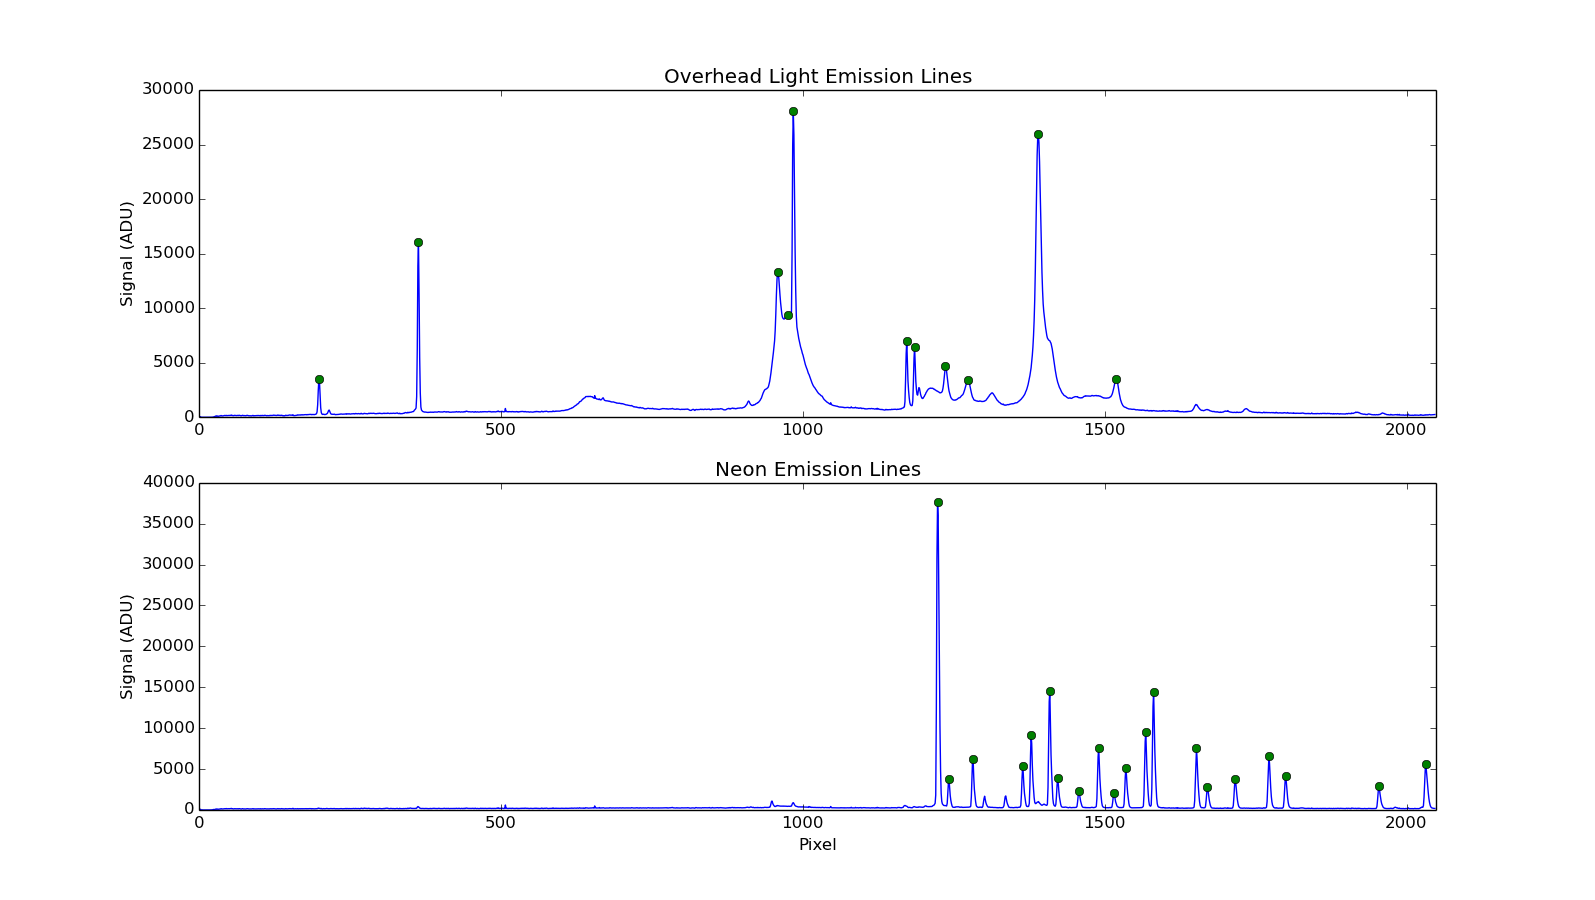
\includegraphics[scale = 0.35]{lab_neon_mercury.png}
\caption{Characteristic emission lines obtained with the lab spectrometer.}
\label{fig:labneon}
\end{figure}

With this comparison, a set of pixel-wavelength points was found. Though initially fit with matrices constructed in Python, it became simpler to use the scipy.optimize,leastsq module to perform the least squares fitting. This method provides a fit for data points by modifying the parameters used in a function of the user's choice so as to minimize the $\chi^2$ value, where:
\begin{equation}
\chi^2= {\sum_{i=1}^{N}{\frac{y_{exp_{i}}-y_{fit_{i}}}{\sigma^2_y}}}
\end{equation}
The other parameters are familiar: N is the number of data points, $y_{exp}$ is the measured data, $y_{fit}$ is the predicted values and $\sigma^2_y$ is the variance in $y_{exp}$. Minimizing this value is the same as minimizing the difference between the experimental points and fitted curve. The division by variance means that experimental values with smaller uncertainty are more heavily weighted.

A linear fit ($\lambda_i=0.427(pixel_i)+383.59$) proved to be adequate for the telescope, but a more complicated fit was necessary for the lab spectrometer (Figure~\ref{fig:solution}). The final polynomial solution had the form of Equation~\ref{eqn:wavesolution}, and a comparison of the calculated values and those supplied by the manufacturer can be found in Table~\ref{tab:polytable}. 
\begin{equation}
\label{eqn:wavesolution}
\lambda_{i}= {\sum_{j=0}^{3}{a_jj^i}}
\end{equation}
\begin{table}[!htbp]
  \centering
  \begin{tabular}{l||l||l||l}
    Constant & Manufacturer Solution & Calculated Solution & Absolute Difference\\
    \hline
    a$_{0}$ & 365.7268923 & 366.868875 & 1.1419827\\
    \hline
    a$_{1}$ & 0.197792654 & 0.197670766 & 1.218880\e{-4}\\
    \hline
    a$_{2}$ & -1.44488\e{-5} & -1.52961\e{-5} & 8.473\e{-7}\\
    \hline
    a$_{3}$ & -5.63994\e{-10} & -2.02471\e{-10} & 3.615\e{-10}\\
    \end{tabular}
    \caption{Comparison between calculated wavlength solution polynomial coefficients and those provided by the manufacturer for the USB 2000 spectrometer.}
    \label{tab:polytable}
\end{table}


\begin{figure}[!htbp]
\centering
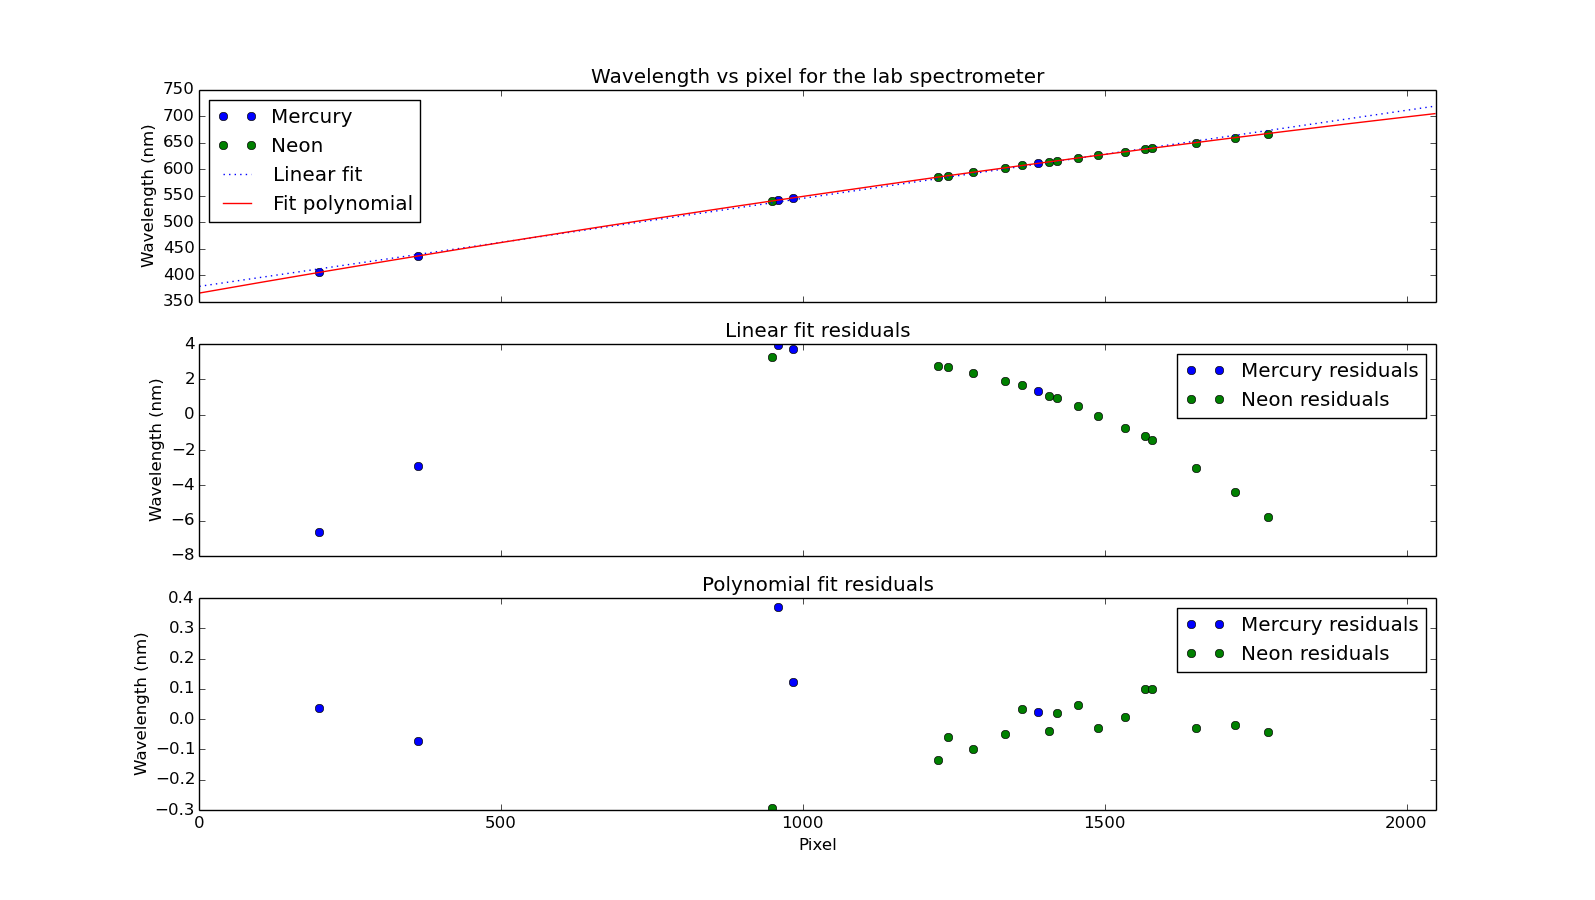
\includegraphics[scale = 0.35]{wavelengthsolution.png}
\caption{Fitting a wavelength solution for the lab spectrometer}
\label{fig:solution}
\end{figure}

The end result was a cubic fit for the lab spectrometer, using the calculated solution constants in Table~\ref{tab:polytable}. Figure~\ref{fig:solution} shows a linear and cubic fit to the data. It is clear from the residuals plots that the linear fit still exhibited order in its deviation from the data points, so a higher order fit was needed. The calculated wavelength solutions were applied to all subsequent spectra. The next step was to further characterize the lab spectrometer. In particular, the saturation level, read noise and gain were calculated. The saturation level was found by experimentation, moving the detector closer to a source until the pixels began to reach a maximum ADU. This value was found to be 65536 ADU, exactly as predicted by the specifications. The gain and read noise calculation was slightly more complicated. It required making a plot of mean value vs variance for a set of observations. The chosen source was the provided desk lamp, and 1024 100 $\mu$s exposures were taken with the detector taped in place. The lamp and detector set up were put into a closest to reduce external influences and the lamp was allowed to run for a few minutes in order to heat up to running temperature. Despite these precautions, there were still overall variations in the ADU recorded by each pixel over time (see Pixel 1349 in Figure~\ref{fig:pixels}).

\begin{figure}[!htbp]
\centering
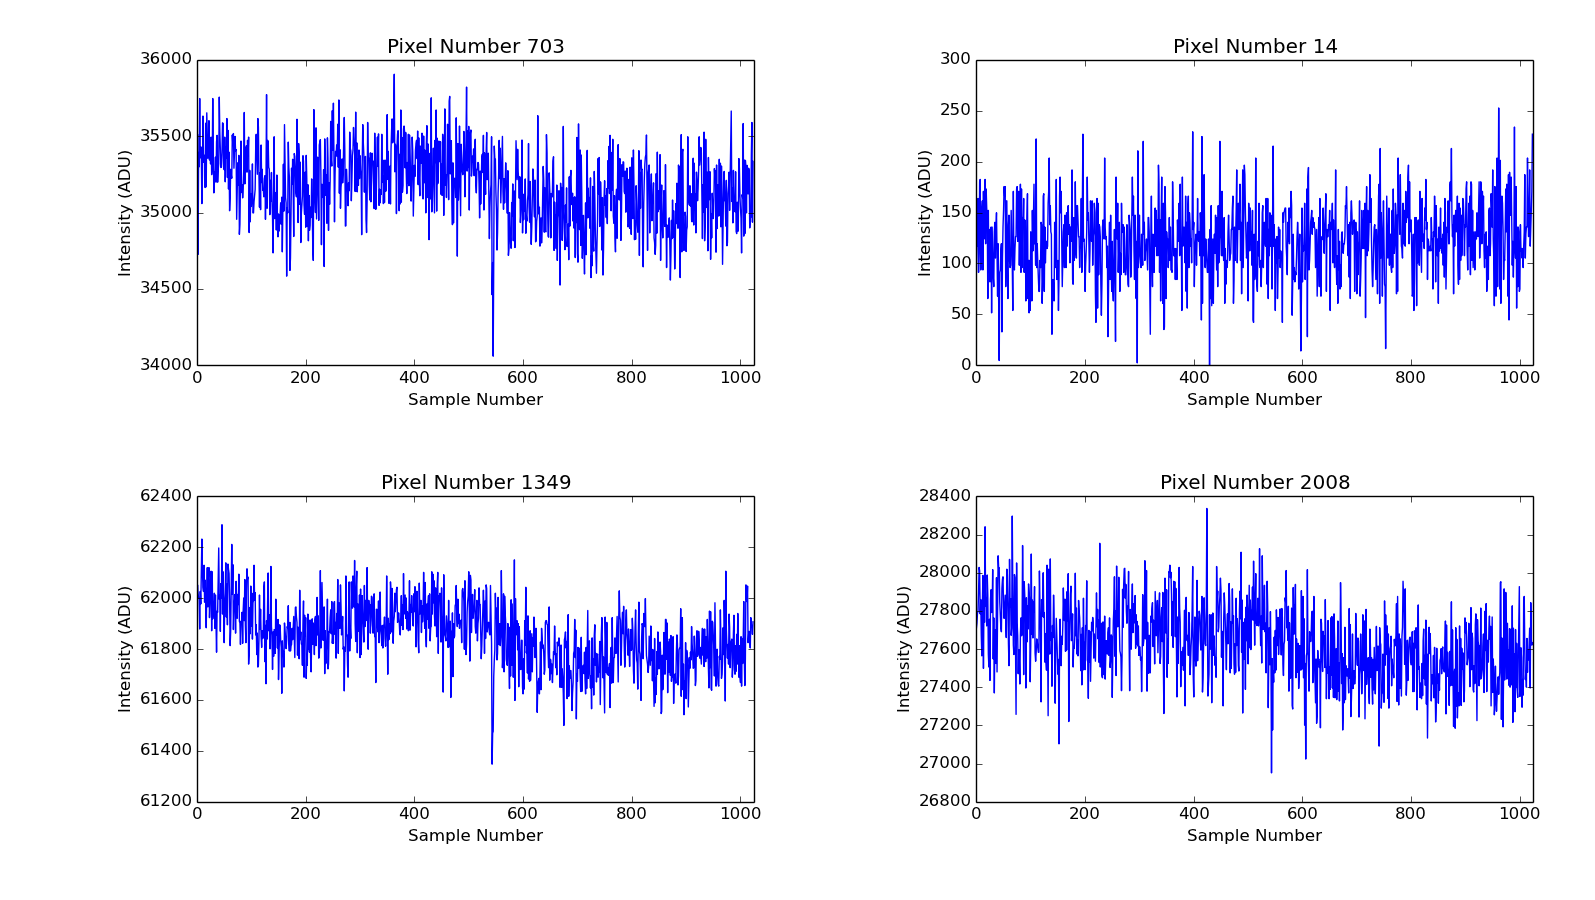
\includegraphics[scale = 0.35]{pixels_vs_samples.png}
\caption{Fluctuations in intensity over a set 1024 100$\mu$s exposures.}
\label{fig:pixels}
\end{figure}

Of these 1024 exposures, exposures 800 to 1000 were selected as being a relatively stable region. The mean and variance of each pixel was calculated and plotted to form the top graph Figure~\ref{fig:gain}. Since the spectrometer counts photoelectrons, one would expect that the mean and variance would display a linear relationship, in accordance with Poisson statistics. Even though the saturation level is 65536 ADU, linear CCD behaviour begins to break down before that (around 40000 ADU). The reasons for this are described in Section~\ref{sec:discussion}. It was sufficient to make a fit to the data from 0 to 40000 ADU, where the points are well behaved. The fit had the form $s^2_{ADU}=s^2_0+kx_{ADU}$, where $s^2_{ADU}$ is the variance of the pixel, $s^2_0$ is the read noise, $k$ is the inverse of the gain and $x_{ADU}$ is the mean ADU value. A slight modification was necessary because the data is also non linear at very low means. The y-intercept of the linear fit is not actually where the data points seem to cross the y-axis. Thus the data was also fitted with a quadratic polynomial, which provided the value of the read noise. Once again using least squares fitting, the gain was found to be 0.8331 $\pm$ 1\e{-5}electrons per ADU, and the read noise 34.52 $\pm$ 0.29 ADU.

\begin{figure}[!htbp]
\centering
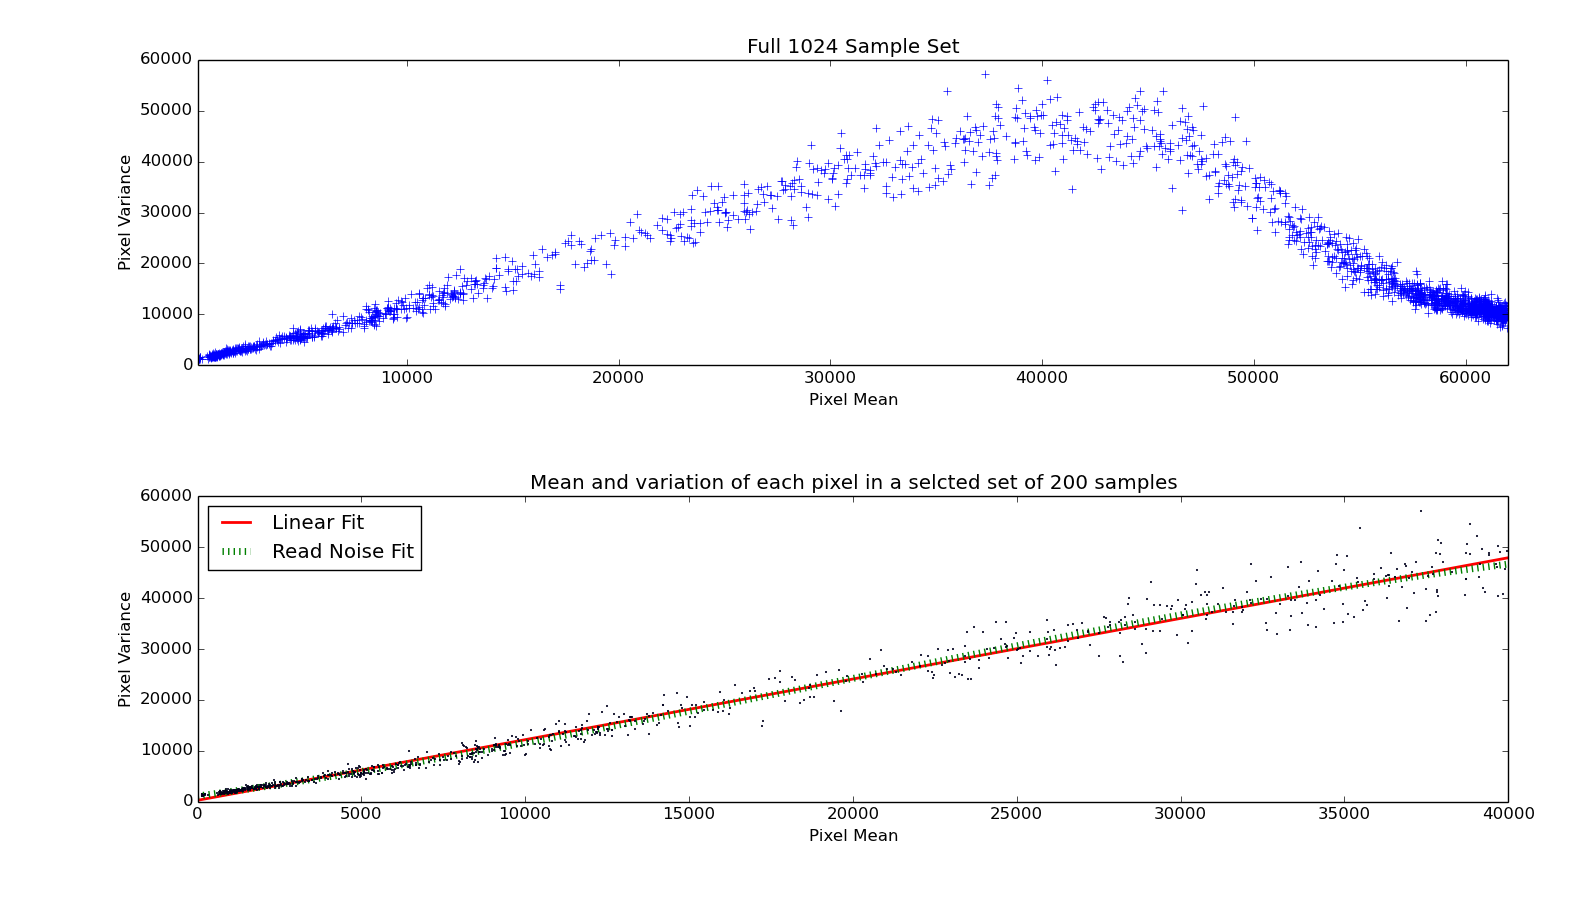
\includegraphics[scale = 0.35]{gain_readnoise2.png}
\caption{Linear fitting of mean ADU vs variance plots to yield gain and read noise of the lab spectrometer. }
\label{fig:gain}
\end{figure}

Parallel to this process of characterizing the lab spectrometer was the analysis of telescope data. The data was a provided in .fit file format as a two dimensional array (see Figure~\ref{fig:vega} for an example of the output). Therefore the primary objective was to extract the information into a more familiar one-dimensional spectra. As is obvious from Figure~\ref{fig:vega}, not all of the spatial dimension was illuminated. The astropy.io.fits python module was used to extract the .fit file as a matrix, then the row with the maximum value was found. This corresponded to a spectrum, and despite some errors where hot pixels were located, resulted in expected output. The ten spectra on either side of this maximum were averaged together to produce a smooth curve (the top plot of Figure~\ref{fig:processed}, for example). Dark subtraction was simple, but another step was required. Namely, accounting for pixel sensitivity with flat fielding with Equation~\ref{eqn:process}.
\begin{equation}
\label{eqn:process}
P_i=\frac{R_i-D_i}{L_i-D_i}B(\lambda_i,T)
\end{equation}
Here, $P_i$ is the processed spectrum pixel, $R_i$ the raw spectrum, $D_i$ the dark spectrum, $L_i$ is the lamp spectrum, and $B(\lambda_i,T)$, the Planck function for a blackbody:
\begin{equation}
\label{eqn:planck}
B(\lambda,T)=\frac{2hc^2}{\lambda^5}\frac{1}{exp(\frac{hc}{Tk_B\lambda})-1}
\end{equation}
Equation~\ref{eqn:planck} depends on the wavelength ($\lambda$), temperature of the blackbody ($T$), Planck's constant ($h$), the speed of light ($c$) and the Boltzman constant ($k_B$). For this experiment, the lamp spectrum used was supposed be for a 3200K bulb, but a quick analysis of the spectra using Wien's law ($\lambda_{peak}T= 2.897\e{-3}m\cdot K$) implied a temperature closer to 4553K. It was this value used to process the spectra.
\section{Discussion}
\label{sec:discussion}

This discussion shall be in two parts: the first concerned solely with characterizing lab spectrometers, the second with the analysis of acquired spectra. The former was, in some senses, the simpler of the two components. Clear instructions were given on the methods of characterizing the spectrometer, it was simply a matter of following them. In the case of the wavelength solution, results correlated remarkably well with expectations. A linear fit to the telescope data, though not plotted here, was very appropriate. It was easy to assume that the spectrometer used on the campus telescope would be more precise than the one in the lab, and a linear fit would be simplest. The lab spectrometer required more work; a polynomial solution was needed. However, this was anticipated by the manufacturers, and the fit values found were all of the same order as the provided solution (Table~\ref{tab:polytable}). The higher order terms are very small, 10\e{-5} and 10\e{-10} times less than the linear term, so overall behaviour is still approximately linear. 

In any case, it was a simple matter to apply this wavelength solution to the raw data and take some initial steps towards spectral analysis. After its application, further properties of the spectrometer could be investigated. Saturation level was another concern, as it limited the intensity of the data recorded. Saturation occurred when the CCD well was full of electrons. Since the CCD pixels record by accepting electrons and transforming them into counts, it is bounded by an upper limit called full well capacity: the maximum number of electrons it can accept. The telescope spectrometer simply resets the pixel count to zero when it reaches this maximum, no longer allowing that pixel to accept photoelectrons. However, the lab spectrometer stops collecting, and remains at that constant, maximum value. This value was easy to measure. Slightly more challenging was understandinging the break down in expected CCD behavior as that value was approached. In Figure~\ref{fig:gain}, the mean and variance per pixel follow the expected linear relation until around 40000 ADU, when the curve suddenly turns over, following an almost quadratic curve back down to lower variances. Consider the trend prior to this point. The mean is increasing, and as it does, variance increases linearly. This is the hallmark of Poisson statistics. However, at high enough means, the standard deviation is limited by the saturation level, which has the effect of lower the variancee. If one were to perfectly saturate the detector, so that pixels were all receiving much more than 65536 ADU, one would expect zero variance, since all fluctuations would occur above the saturation level. At low means, Figure~\ref{fig:gain} exhibits nonlinear behavior again, but for a different reason. As the mean ADU decreases, it approaches a lower limit in the form of the noise floor \citep{ccd}. This limit is the read noise, and comes from the fact that counts are added to the data by the process of reading them in. Rather than follow its linear behavior all the way to zero, the curve flattens against this lower limit, with the effect of increasing the variance. It was for this reason that two fits were used on the curve: one to estimate the linear behavior, the other to find this lower limit. In this case, it presented as a read noise of 34.52 ADU, on order with typical read noise values \citep{telescopes}, though a bit large. The linear fit gave the gain as the inverse of the slope, equal to 0.83307 electrons per ADU. Since the gain is the number of electrons needed to produce 1 ADU, this doesn’t seem to be correct. One would expect an average of one or more electrons needed to produce one count.

It is highly likely that even though a small and relatively steady interval was selected from the set of exposure used to make this plot, some overall trend produced distortions in the data. The fit also might have been improved by having more points in the region of means less than 40000 ADU. However, five separate trials with multiple selections from each failed to remove this effect. The detector sensitivity simply allows for high value of fluctuation. 
\begin{figure}[!htbp]
\centering
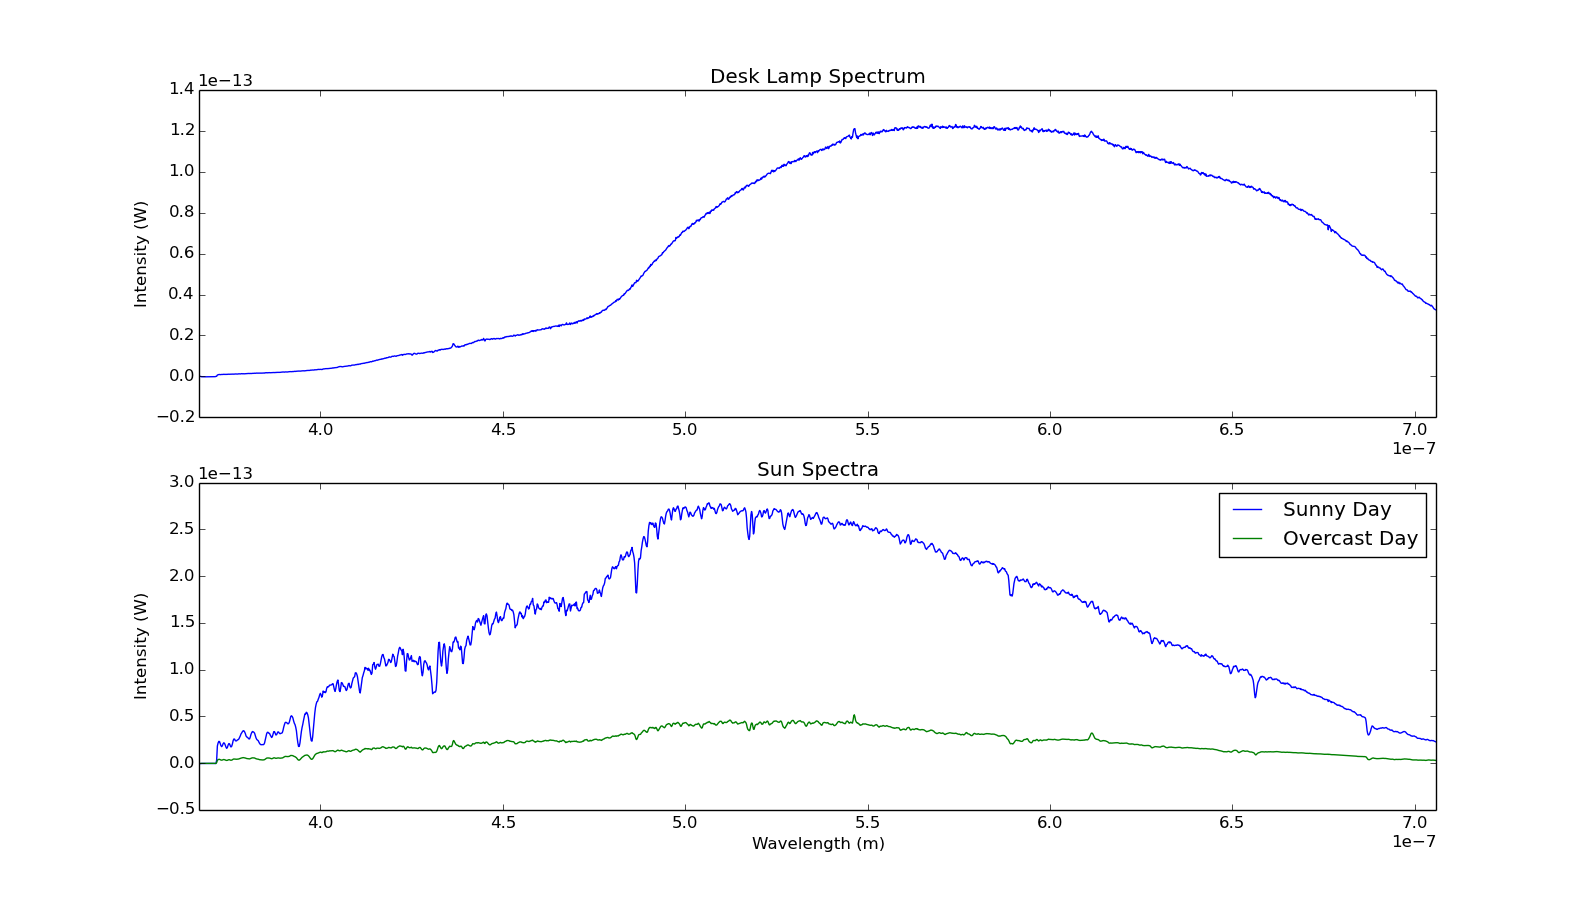
\includegraphics[scale = 0.35]{lab_spec.png}
\caption{Two spectra taken with the lab spectrometer. Both have been corrected for the gain and read noise and converted from ADU to energy per second.}
\label{fig:labspec}
\end{figure}
The read noise was subtracted from the lab data to remove the noise floor, and the gain was used to convert from ADU to electrons. From there, it was a matter of assuming that each electron at a particular wavelength $\lambda$ represented a photon with energy $E=\frac{hc}{\lambda}$ to find the total energy at each wavelength. This value was converted to power by dividing by the exposure time, to create plots like Figure~\ref{fig:labspec}.

\begin{figure}[!htbp]
\centering
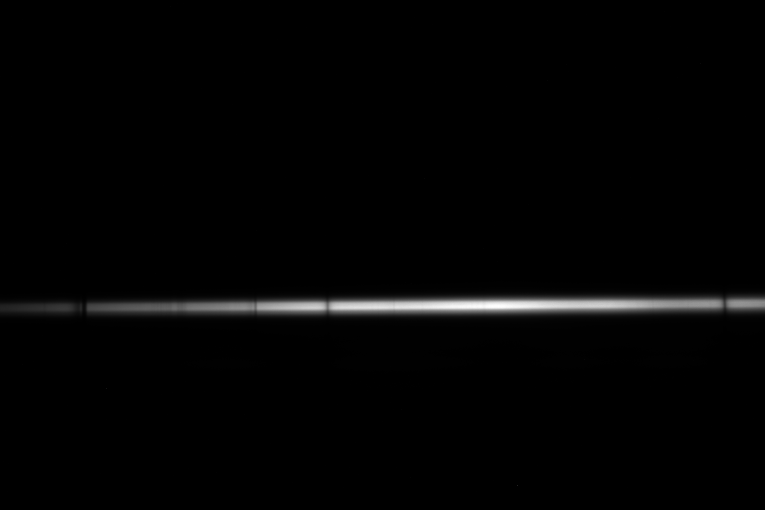
\includegraphics[width=\linewidth,height=0.5in]{vega.png}
\caption{Raw output from the telescope spectrometer. This image is of Vega. Horizontal pixels are dispered wavelength intensity, vertical pixels represent the spatial dimension.}
\label{fig:vega}
\end{figure}

The data from the telescope was also processed, according to the method outlined in Section~\ref{sec:calc}. This changed a two dimensional spectrum like Figure~\ref{fig:vega} to a more comprehensible spectrum like Figure~\ref{fig:processed}. Similar steps were taken with the other stellar sources to produce Figure~\ref{fig:bin}.

\begin{figure}[!htbp]
\centering
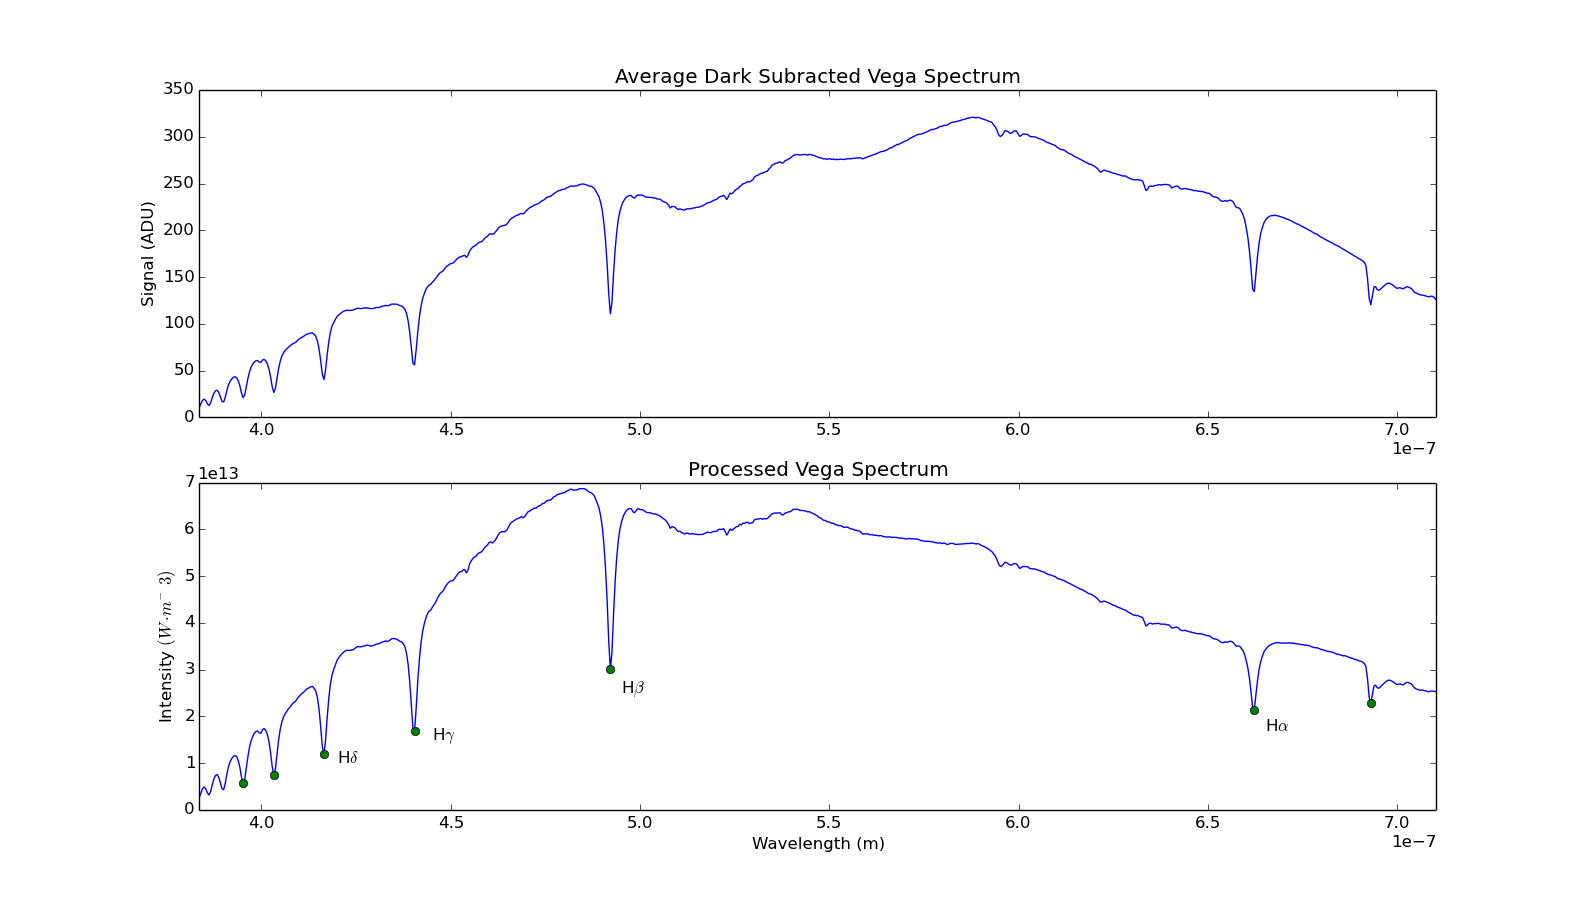
\includegraphics[scale = 0.35]{processed_vega.png}
\caption{Processing steps applied to Vega spectra taken on the first night. Balmer hydrogen emission lines are labelled.}
\label{fig:processed}
\end{figure}
Applying Wien’s Law to the processed stellar spectra produced strange results (see Table~\ref{tab:sources}), not at all matching expecations. It can only be assumed that something went wrong during the processing step, though it is not clear what exactly that was. The only thing that matches well is the sun temperature, which was measured with the lab spectrometer and not processed like the others.
\begin{table}[!htbp]
  \centering
  \begin{tabular}{p{1in}||p{1in}||p{1in}||p{1in}||p{1in}}
    Source & Expected Temperature & Spectrum Temperature & Implied Spectral Type & Actual Spectral Type\\
    \hline
    Sun & 5778K  & 5722K & G & G\\
    \hline
    Vega & 9500K \citep{vega} & 5976K & G & A\\
    \hline
    Enif & 4460K \citep{enif} & 4918K & K & K\\
    \hline
    Albireo A (Albireo 2) & 4080K \citep{albireo} & 6050K & F & K\\
    \hline
    Albireo B (Albireo 1) & 13200K \citep{albireo} & 6810K & F & B\\
    \end{tabular}
    \caption{Comparison between expected source surface temperature and those produced with Wien's Law.}
    \label{tab:sources}
\end{table}
The precise nature of the problem is not immediately evident, as the processing step was followed exactly, using the same exposure times and a temperature derived from the lamp spectrum itself. If the lamp spectrum were a perfect blackbody, the process would do nothing at all, since it would simply divide and multiply by the blackbody function. It is the lamp spectrum imperfections that are taken to be indicative of pixel sensitivity. The Vega spectrum, with both before and after images (Figure~\ref{fig:processed}) provides an example. Here, the processing step has blue-shifted the peak, as would be expected. However, the shift is not as far as anticipated.
\begin{figure}[!htbp]
\centering
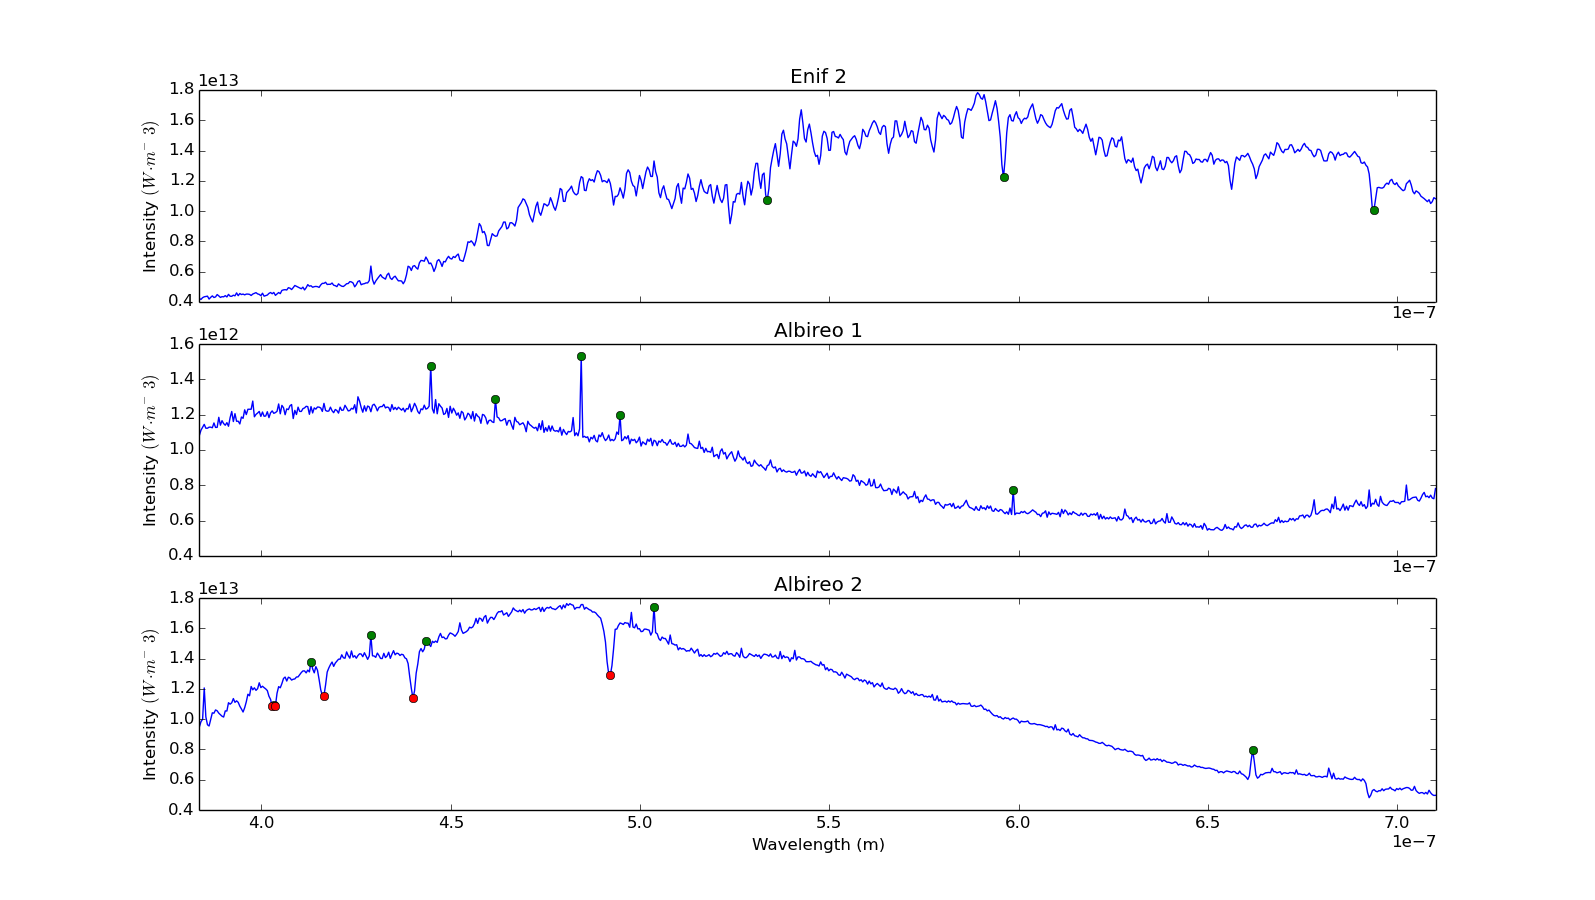
\includegraphics[scale = 0.35]{telescope_binaries2.png}
\caption{Three processed stellar spectra taken wih the campus telescope.}
\label{fig:bin}
\end{figure}
In addition to determining spectral type, emission and absorption features were investigated. These appear when light of certain wavelength is emitted or absorbed in excess of its fellows. Photons of particular wavelengths represent the transition of electrons between orbitals for specific elements or ions. For the sun spectrum, it is easy to see characteristic absorption features: two $Ca^+$ ion features near 400nm, an Fe absorption line around 450nm, Na around 600nm and an $O_2$ feature around 700nm. $H\alpha$ and $H\beta$ lines are also visible. Hydrogen lines can also be seen in the Vega and Albireo 2 spectra, though in this case far more of them are obvious: $H\beta$ through $H\delta$ as well as the Balmer jump, which presents as a series of dips at low wavelengths. The $H\alpha$ feature appears in Vega and Enif.

The characteristics of these hydrogen lines were investigated quantitatively in the Vega spectrum, and it was found that the location of the lines are redshifted from the expected values by about 7nm \citep{hlines}. This does not necessarily imply inaccuracy of the wavelength solution. It may, in fact, be a result of Vega's movement with respect to the earth. Vega displays the $O_2$ feature as well, and it also appears in the Albireo 2 and Enif spectra. The Albireo 1 spectrum's features mostly appear as emission spikes, mostly located around the $H\alpha$, $H\beta$ and $H\gamma$ wavelengths.

Though these absorption features make sense, the temperature characterization does not. Stars are expected to be reasonably good blackbodies. Spectra exhibit spiky emission and absorption lines, but they have an overall smooth curve, the peak of which occurs at a wavelength that determines the temperature according to Wien’s law. This was not found to be the case, and so more investigation is needed.

Although the results of this lab were at times unexpected, the theory needed to access them will doubtless prove useful in future astronomical endeavors. The nature of the processing steps used on the telescope spectra bear further scrutiny, as some step in that procedure produced unexpected results.

\bibliographystyle{plainnat}
\bibliography{cite}

\end{document}